\documentclass[a4paper,12pt]{article} 

% First, we usually want to set the margins of our document. For this we use the package geometry.
\usepackage[top = 2.5cm, bottom = 2.5cm, left = 2.5cm, right = 2.5cm]{geometry} 
\usepackage[T1]{fontenc}
\usepackage[utf8]{inputenc}

% The following two packages - multirow and booktabs - are needed to create nice looking tables.
\usepackage{multirow} % Multirow is for tables with multiple rows within one cell.
\usepackage{booktabs} % For even nicer tables.

% As we usually want to include some plots (.pdf files) we need a package for that.
\usepackage{graphicx} 

% The default setting of LaTeX is to indent new paragraphs. This is useful for articles. But not really nice for homework problem sets. The following command sets the indent to 0.
%\usepackage{setspace}
%\setlength{\parindent}{0in}
\usepackage{indentfirst}

% Package to place figures where you want them.
\usepackage{float}

% The fancyhdr package let's us create nice headers.
\usepackage{fancyhdr}

\usepackage{amsmath,amsthm,tikz}
\usetikzlibrary{automata,positioning,patterns}

% To make our document nice we want a header and number the pages in the footer.

\pagestyle{fancy} % With this command we can customize the header style.

\fancyhf{} % This makes sure we do not have other information in our header or footer.

\lhead{\footnotesize Data Structure and Algorithm Analysis(H): Work Sheet 14}% \lhead puts text in the top left corner. \footnotesize sets our font to a smaller size.

%\rhead works just like \lhead (you can also use \chead)
\rhead{\footnotesize Mengxuan Wu} %<---- Fill in your lastnames.

% Similar commands work for the footer (\lfoot, \cfoot and \rfoot).
% We want to put our page number in the center.
\cfoot{\footnotesize \thepage} 

\begin{document}

\thispagestyle{empty} % This command disables the header on the first page. 

\begin{tabular}{p{15.5cm}}
{\large \bf Data Structure and Algorithm Analysis(H)} \\
Southern University of Science and Technology \\ Mengxuan Wu \\ 12212006 \\
\hline
\\
\end{tabular}

\vspace*{0.3cm} %add some vertical space in between the line and our title.

\begin{center}
	{\Large \bf Work Sheet 14}
	\vspace{2mm}

	{\bf Mengxuan Wu}
		
\end{center}  

\vspace{0.4cm}

\section*{Question 14.1}

\begin{center}
	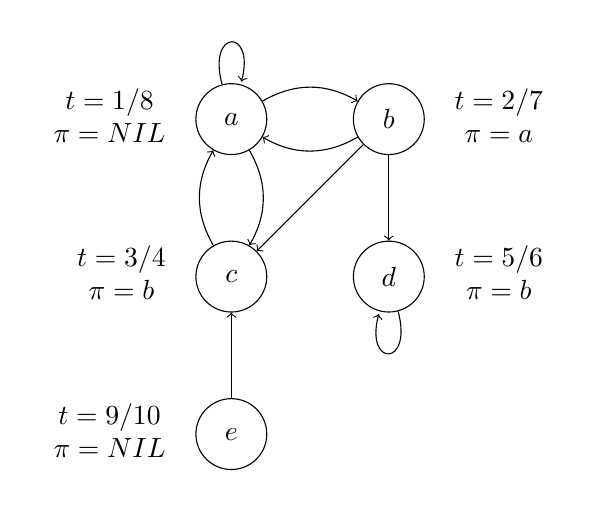
\begin{tikzpicture}
		\draw (0,0) node [circle,draw, minimum size=0.9cm] (a) {$a$};
		\draw (-0.5,0) node [left] {\begin{tabular}{c} $t = 1 / 8$ \\ $\pi = NIL$ \end{tabular}};
		\draw (2,0) node [circle,draw, minimum size=0.9cm] (b) {$b$};
		\draw (2.5,0) node [right] {\begin{tabular}{c} $t = 2 / 7$ \\ $\pi = a$ \end{tabular}};
		\draw (0,-2) node [circle,draw, minimum size=0.9cm] (c) {$c$};
		\draw (-0.5,-2) node [left] {\begin{tabular}{c} $t = 3 / 4$ \\ $\pi = b$ \end{tabular}};
		\draw (2,-2) node [circle,draw, minimum size=0.9cm] (d) {$d$};
		\draw (2.5,-2) node [right] {\begin{tabular}{c} $t = 5 / 6$ \\ $\pi = b$ \end{tabular}};
		\draw (0,-4) node [circle,draw, minimum size=0.9cm] (e) {$e$};
		\draw (-0.5,-4) node [left] {\begin{tabular}{c} $t = 9 / 10$ \\ $\pi = NIL$ \end{tabular}};
		\path[->]
			(a) edge [bend left] (b)
			    edge [loop above] (a)
				edge [bend left] (c)
			(b) edge [bend left] (a)
			    edge (c)
				edge (d)
			(c) edge [bend left] (a)
			(d) edge [loop below] (d)
			(e) edge (c);
	\end{tikzpicture}
\end{center}

\section*{Question 14.2}

\begin{proof}[Disproof]
$ $

No.
The number of back edges might change because one back edge can participate in multiple cycles.

Consider the following graph:
\begin{center}
	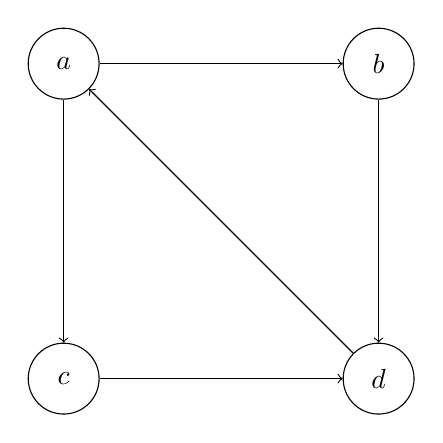
\begin{tikzpicture}[nodes={draw, circle, minimum size=0.9cm}]
		\draw (0,0) node (a) {$a$};
		\draw (4,0) node (b) {$b$};
		\draw (0,-4) node (c) {$c$};
		\draw (4,-4) node (d) {$d$};
		\path[->]
			(a) edge (b)
				edge (c)
			(b) edge (d)
			(c) edge (d)
			(d) edge (a);
	\end{tikzpicture}
\end{center}

\newpage
If we run DFS on vertex $a$, we will get the following DFS tree:
\begin{center}
	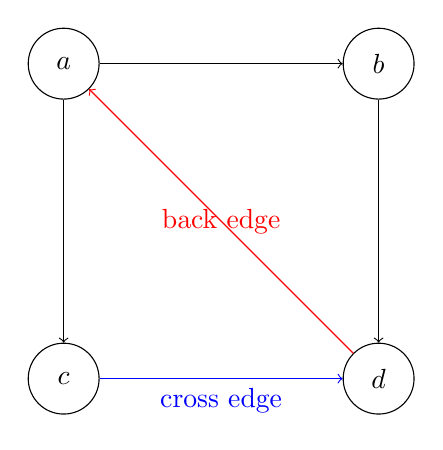
\begin{tikzpicture}
		\draw (0,0) node [draw, circle, minimum size=0.9cm] (a) {$a$};
		\draw (4,0) node [draw, circle, minimum size=0.9cm] (b) {$b$};
		\draw (0,-4) node [draw, circle, minimum size=0.9cm] (c) {$c$};
		\draw (4,-4) node [draw, circle, minimum size=0.9cm] (d) {$d$};
		\path[->]
			(a) edge (b)
				edge (c)
			(b) edge (d)
			(c) edge [blue] node [below] {cross edge} (d)
			(d) edge [red] node {back edge} (a);
	\end{tikzpicture}
\end{center}

If we run DFS on vertex $b$, we will get the following DFS tree:
\begin{center}
	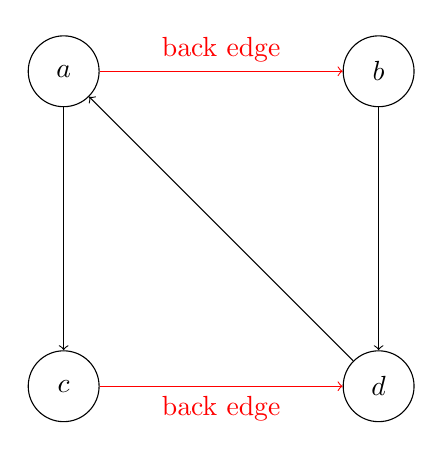
\begin{tikzpicture}
		\draw (0,0) node [draw, circle, minimum size=0.9cm] (a) {$a$};
		\draw (4,0) node [draw, circle, minimum size=0.9cm] (b) {$b$};
		\draw (0,-4) node [draw, circle, minimum size=0.9cm] (c) {$c$};
		\draw (4,-4) node [draw, circle, minimum size=0.9cm] (d) {$d$};
		\path[->]
			(a) edge [red] node [above] {back edge} (b)
				edge (c)
			(b) edge (d)
			(c) edge [red] node [below] {back edge} (d)
			(d) edge (a);
	\end{tikzpicture}
\end{center}
\end{proof}

\section*{Question 14.3}

\begin{center}
	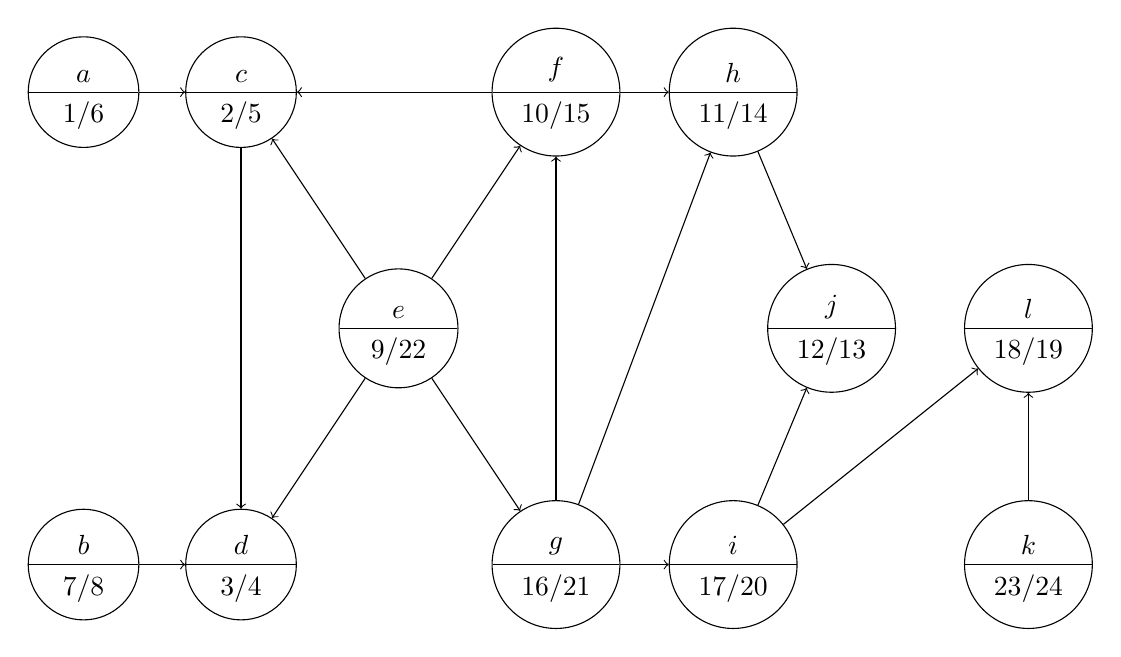
\begin{tikzpicture}[auto]
		\draw (0,0) node [state with output] (a) {$a$ \nodepart{lower} 1/6};
		\draw (0,-6) node [state with output] (b) {$b$ \nodepart{lower} 7/8};
		\draw (2,0) node [state with output] (c) {$c$ \nodepart{lower} 2/5};
		\draw (2,-6) node [state with output] (d) {$d$ \nodepart{lower} 3/4};
		\draw (4,-3) node [state with output] (e) {$e$ \nodepart{lower} 9/22};
		\draw (6,0) node [state with output] (f) {$f$ \nodepart{lower} 10/15};
		\draw (6,-6) node [state with output] (g) {$g$ \nodepart{lower} 16/21};
		\draw (8.25,0) node [state with output] (h) {$h$ \nodepart{lower} 11/14};
		\draw (8.25,-6) node [state with output] (i) {$i$ \nodepart{lower} 17/20};
		\draw (9.5,-3) node [state with output] (j) {$j$ \nodepart{lower} 12/13};
		\draw (12,-6) node [state with output] (k) {$k$ \nodepart{lower} 23/24};
		\draw (12,-3) node [state with output] (l) {$l$ \nodepart{lower} 18/19};
		\path[->]
			(a) edge (c)
			(b) edge (d)
			(c) edge (d)
			(e) edge (c)
				edge (d)
				edge (f)
				edge (g)
			(f) edge (c)
				edge (h)
			(g) edge (f)
			    edge (h)
				edge (i)
			(h) edge (j)
			(i) edge (j)
			    edge (l)
			(k) edge (l);
	\end{tikzpicture}
\end{center}

The list sorted by finishing time is: $k, e, g, i, l, f, h, j, b, a, c, d$.

\section*{Question 14.4}

\begin{center}
	\begin{tabular}{ll}
		\toprule
		\multicolumn{2}{c}{\textsc{Check-Is-Acyclic}($G(V, E)$)} \\
		\midrule
		1 & \textbf{if} $|E| > |V| - 1$ \\
		2 & \qquad \textbf{return} \textsc{False} \\
		3 & \textsc{DFS'}($G(V, E)$) \\
		4 & \textbf{for} each edge $(u, v) \in E$ \\
		5 & \qquad \textbf{if} $(u, v) \text{ is a back edge}$ \\
		6 & \qquad \qquad \textbf{return} \textsc{False} \\
		7 & \textbf{return} \textsc{True} \\
		\bottomrule
	\end{tabular}
\end{center}

For an undirected graph, if there is no cycle in the graph, then it must be a tree or a forest. 
And for a tree or a forest, $|E| \leq |V| - 1$ must be true.
Hence, we check this condition first.
If the condition is not satisfied, we return \textsc{False} immediately and runtime is $O(1)$.

If the condition is satisfied, we run DFS on the graph.
Here we can modify the DFS algorithm to explicitly mark each back edge, since it only takes $O(1)$ time, the runtime of DFS is still $O(|V| + |E|)$.
Then, we check each edge in the graph.

The runtime of DFS is $O(|V| + |E|)$.
Since we know $|E| \leq |V| - 1$, we can infer that $O(|V| + |E|) = O(|V|)$.
Then, the total runtime of the algorithm is $O(|V|) + O(|V|) = O(|V|)$.

Hence, in any case, the runtime of the algorithm is $O(|V|)$.
\end{document}